% !TEX root = approx8.tex


	We split the proofs of the two geometric situations into subsections. The basic idea is the same: cut the ambient manifold into more and more equally spaced straight slices. We will keep on writing Fukaya categories as $\mathcal{A}_p$ and systems of Fukaya categories as $\widehat{\mathcal{A}}$ as indicated at the beginning of Section \ref{sec:split-app}.
\subsubsection{Approximability of equators on the $2$-sphere} In what follows we will refer to a closed monotone Lagrangian $L\subset S^2$ as an "equator". Note that these Lagrangians are precisely the embedded curves in $S^2$ which separate it into two domeains of equal area.

The first Chern class of $S^2$ vanishes in $H^2(S^2;\mathbb{Z}_2)$, so the eigenspace of the quantum homology $QH(S^2,\Lambda)$ associated to the zero eigenvalue is the whole space. \\ In this subsection, we will only consider (without loss of generality) perturbation data $p\in \mathcal{P}$ satisfying the following two conditions:
\begin{enumerate}
	\item Let $L\in \lag^{\text{(mon,} \mathbf{0} \text{)}}(S^2)$ be an equator on $S^2$ and consider the Morse function $f^L_p\colon L\to \mathbb{R}$ in the $p$-Floer datum of $L$. We assume that $f^L_p$ has a unique maximum $e_L\in L$ and a unique minimum $\text{pt}_L\in L$. We will always assume that both $e_L$ and $\text{pt}_L$ are neither the north nor south poles of $S^2$.
	\item Consider the Morse function $f^{S^2}_p\colon S^2\to \mathbb R$ in the $p$-Floer datum for $S^2$. We assume that $f^{S^2}_p$ has a unique maximum $u_{S^2}\in S^2$ and a unique minimum $\text{pt}_{S^2}\in S^2$ and no other critical points. We further assume that both $u_{S^2}$ and $\text{pt}_{S^2}$ differ from both the north and south poles of $S^2$, 
\end{enumerate}
We will abuse notation and write this "restriction" of $\mathcal{P}$ again as $\mathcal{P}$ and consider the homotopy system of $A_\infty$-categories $\widehat{\mathcal{A}}= \widehat{\fuk}(\lag^{\text{(mon,} \mathbf{0} \text{)}}(S^2))$ as parametrized by this restricted $\mathcal{P}$.
\begin{prop}\label{singlelagsphere}
	Let $L\in \lag^{\text{(mon,} \mathbf{0} \text{)}}(S^2)$ be an equator on $S^2$. Then $\lag^{\text{(mon,} \mathbf{0} \text{)}}(S^2)$ is $\frac{1}{4}$-retract approximable by $L$.
	%for any perturbation datum $p\in E^{sg}$, the open closed-map $OC_p^L\colon HH(L,L)\to QH(S^2)$ satisfies $R(u_{S^2},OC_p^L)\leq \frac{1}{2$}$. {\color{orange} Maybe write it as "Then, for any perturbation datum $p\in E^\mu$ we have $$R(u,OC_p^L)=\frac{1}{2}.$$}
\end{prop}

\begin{proof}
	%We assume that the Morse function $f_L$ associated to the Floer datum of $p$ on $L$ is the height function. Denote by $e_L$ the maximum of $f_L$ and by $\text{pt}_L$ its minumum. Then $CF(L,L)= \Lambda\cdot e_L\oplus \Lambda\cdot \text{pt}_L$. As above, we will work with the height function $f_{S^2}$ on the sphere to define quantum homology, which has a unique maximum $u_{S^2}$ and a unique minumim $\text{pt}_{S^2}$. In particular $CQ(M) = \Lambda\cdot u_{S^2}\oplus \text{pt}_{S^2}$.\\
	%Consider the length filtration $(F^NCC_*(L,L))$ on the Hochschild chain complex as introduced in Section \ref{persistencehochschild}, and the restristion $F^1OC_p^L$ of the chain-level open closed map to $F^1CC_*(L,L)$.
	Let $p\in \mathcal{P}$. It is easy to see
	%that $$OC_p^L(\text{pt}_L\otimes e_L) = OC_p^L(e_L\otimes \text{pt}_L) = OC_p^L(e_L\otimes e_L) = 0 $$
	that at the chain level we have $$OC_p^L(\text{pt}_L\otimes \text{pt}_L) = T^{\frac{1}{2}}u_{S^2}.$$ Moreover, since $d_{CC}$ is cyclic, $\text{pt}_L\otimes \text{pt}_L$ is a cycle in $CC_*(L,L)$. Note that the persistence Hochschild homology $PHH_*(L_p)$ does not depend on $p\in \mathcal{P}$. The claim then follows by Theorem \ref{gio:wabomain}.
	%All of the listed elements in $F^1CC(L,L)$ are cycles as $d_{CC}$ is cyclic. The reason behind the fact that there is no $\text{pt}_{S^2}$ contribution in $OC_p^L(\text{pt}_L\otimes \text{pt}_L)$ has to do with transversality of pearly trajectories; for the same reason that there is no ${\text{pt}}_{S^2}$ contribution in the quantum product ${\text{pt}}_{S^2}*{\text{pt}}_{S^2}= Tu_{S^2}$. {\color{orange} see appendix B for the converse.}
\end{proof}
\begin{rem}
a. We actually proved that for a single equator the constant $\delta>0$ appearing in Definition \ref{d:approx-sys-ret} can be taken to be arbitrarily big. This is due to the fact that for the self-Floer homology of $L$ we do not need any Hamiltonian perturbation.

b. The linear component $ HF(L,L)\to QH(S^2)$ of the open-closed map does not hit the unit in our setting: indeed $OC(e_L)=0$ by a degree argument while $OC(\text{pt}_L) = \text{pt}_{S^2}+T^{\frac{1}{2}}u_{S^2}$. Note however, that if we would have worked with coefficients in the Novikov field over the real numbers, the situation would have been different, as $T^{-1\frac{1}{2}}\text{pt}_{S^2}+u_{S^2}$ is the projection of the unit in the zero eigensummand of quantum homology of $\mathcal{C}P^1$ over this coefficient field.\\ Note that as $\text{pt}_{S^2}+T^{\frac{1}{2}}u_{S^2}$ and $u_{S^2}$ are non-homologous cycles in $CQ(S^2)$, it follows that $[\text{pt}_{L}]$ and $[\text{pt}_{L}\otimes \text{pt}_{L}]$ generate $HH(L)$.

c. As we know that $OC^L\colon HH(L)\to QH(S^2)$ is an isomorphism, it follows from the computation above that $e_L\in PHH^\infty(L,L)$ has to be a boundary. In fact, it equals $T^{-\frac{1}{2}}d_{CC}(a_L\otimes a_L\otimes a_L)$, where $a_L = \text{pt}_L+T^{\frac{1}{4}}e_L$; indeed notice that $a_L\in CF(L,L)$ is a cycle satisfying $$\mu_k(a_L,\ldots, a_L) =T^{\frac{1}{2}}e_L \text{  for any }k\geq 2.$$
Hence, $[e_L]$ has boundary depth $\frac{1}{2}$ in $PHH(L)$. Note that $[e_L\otimes \text{pt}_L]$ also has boundary depth equal to $\frac 12$. Indeed $$d_{CC}(a_L^{\otimes 4}) = T^{\frac{1}{2}}(e_L\otimes \text{pt}_L + \text{pt}_L\otimes e_L)$$ and $\text{pt}_L\otimes e_L = d_{CC}(\text{pt}_L\otimes e_L\otimes e_L)$.% This behaviour is further studied in \TBD.
\end{rem}

We will now show that we can approximate the Fukaya category of $S^2$ with better accuracy by considering larger approximating families. Fix an equator $S^1\subset S^2$ as a reference and consider the set $\mathcal{E}\subset \lag^{\text{(mon,} \mathbf{0} \text{)}}(S^2)$ great circles which pass trough the north $n\in S^2$ and south pole $s\in S^2$. %We will pick the orientation on each $L\in \mathcal{E}$ obtained by clockwise rotations of $S^1$ looking from the north pole. 
Of course, any two Lagrangians in $\mathcal{E}$ intersect transversally. Recall that in our setting, given a perturbation datum $p\in \mathcal{P}$, the Hamiltonian part of the $p$-Floer datum associated to a pair $(L_0,L_1)$ of transversally intersecting Lagrangians is assumed to be constant (see page \pageref{gio:FD}), and this constant is $<\nu(p)$, the size of $p$, by definition. Moreover, we require $H^{L_0,L_1}_p=H^{L_1,L_0}_p$. Hence the Floer complexes $CF(L_0,L_1;p)$ and $CF(L_1,L_0;p)$ are generated by the (finitely many) intersection points in $L_0\cap L_1$, and these lie at the same filtration level. Suppose $L_1\in \mathcal{E}$ is obtained by rotating another equator $L_0\in \mathcal{E}$ by an angle smaller than $\pi$. Of course, $L_0\cap L_1$ consists of the north and south poles only: we work with the convention that in the complex $CF(L_0,L_1;p)$ the north pole $n_{0}\in CF(L_0,L_1;p)$ has grading $1$ and the south pole $s_{0}\in CF(L_0,L_1;p)$ has grading $0$, while in the complex $CF(L_1,L_0;p)$ this is viceversa (and the poles are denoted by $n_{1}$ and $s_{1}$ in this complex).

The relevant notion of approximability for the next result is the retract version of Definition \ref{def:simple_approx}.
\begin{prop}\label{OCS2}
	Let $p\in \mathcal{P}$ and $N\geq 2$. Consider a finite family of great circles $\mathcal{E}(N)=\{L_1,\ldots, L_N\}\subset \mathcal{E}$ on $S^2$, all passing through the north and south poles and such that $L_i$ lies at angle difference $\frac{\pi}{2N}$ from $L_{i+1}$. Then $\lag^{\text{(mon,} \mathbf{0} \text{)}}(S^2)$ is retract-approximable in $\mathcal{A}_p$ by the family $\mathcal{E}(N)$ with accuracy $\frac{1}{4N}+2\nu(p)$.
	%{\tiny $$OC^{\mathcal{E}(N)}_p\colon HH^{\leq \frac{1}{2N} + 2\varepsilon}(\mathcal{E}(N))\to QH(S^2)$$ hits the unit. Moreover, given any subfamily $\tilde{\mathcal{B}}$ of cardinality $N$ and any $\alpha< \frac{1}{2N}+2\varepsilon$, the map $$OC^{\tilde{\mathcal{B}}}_p\colon HH^{\leq \alpha}(\tilde{\mathcal{B}})\to QH(S^2)$$ does not hit the unit. {\color{orange} see orange comment in above prop}}
\end{prop}
\begin{figure}
	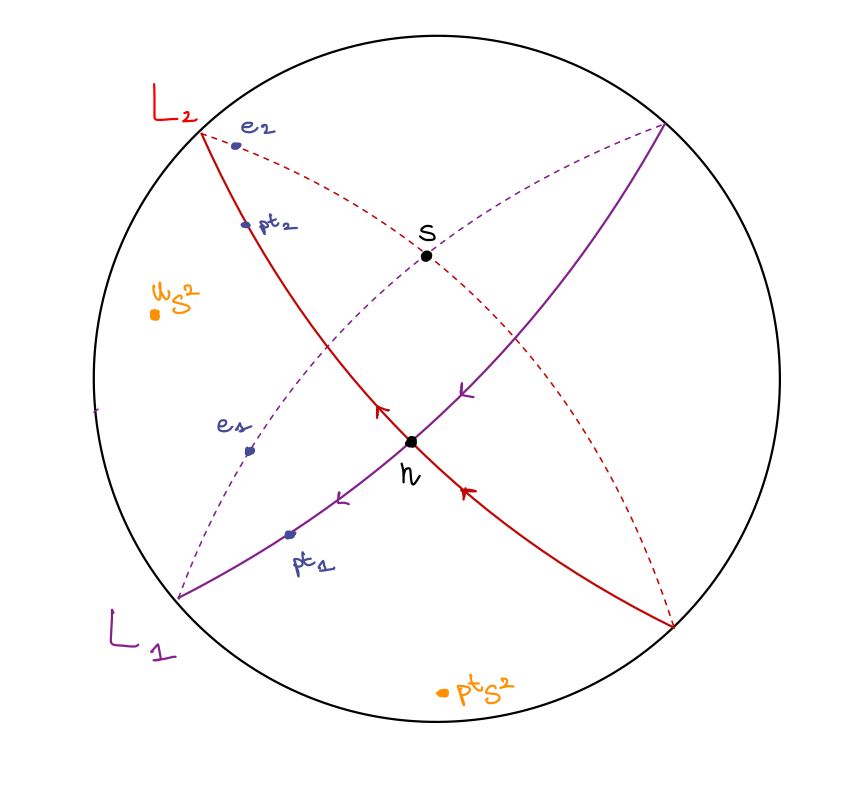
\includegraphics[scale=0.3]{S2approx.png}
	\centering
	\caption{The geometric situation described in Proposition \ref{OCS2} in the case $N=2$.} \label{fig:S2approx}
\end{figure}
\begin{rem}
\begin{proof}
	%Recall that the $p$-Floer complex of any two transversally intersecting Lagrangians is generated by their intersection points, all set at action $\nu(p)$ by definition of our class of Floer data (see Definition \ref{FD}).
	We will number our equators so that looking from the north pole, they are ordered clockwise starting from $L_1$. We drop $p$ from the notation and write $C_i:=CF(L_{i},L_{i+1})$ and $C_i':= CF(L_{i+1},L_i)$ for any $i=1,\ldots, N$\footnote{With the convention $L_{N+1}=L_1$.}. For any $i$, we denote by $n_i, s_i \in C_i$  and $n_i',s_i'\in C_i'$ the north and south poles respectively. To simplify the computations in the remainings of the proof, we impose the following additional restrictions on the functions $f^{L_i}_p$ in the $p$-Floer datum of each equator $L_i$: we require that flowing from the north pole to the south pole, one encounters first $\text{pt}_i$ and then $e_i$, before getting to the south pole. We also require that the critical points $u_{S^2}$ and $\text{pt}_{S^2}$ of the Morse function $f^{S^2}_p$ in the $p$-Floer datum of the ambient manifold $f_p^{S^2}\colon S^2\to \mathbb{R}$ both lie in the area between $L_1$ and $L_2$, but not on $L_1$ or $L_2$.
	
	We claim that $$\vec{\gamma}:=\sum_{i=1}^N n_i\otimes s_i'\in \bigoplus_{i=1}^N C_i\otimes C_i'\subset CC_*(\mathcal{E}(N))$$ is a Hochschild cycle, and moreover $$OC_p^{\mathcal{E}(N)}\left(\sum_{i=1}^N n_i\otimes s_i'\right)=T^{\frac{1}{2N}}u_M.$$ This would prove the statement as $$\mathbb{A}_{CC}\left(\sum_{i=1}^N n_i\otimes s_i'\right) = \mathbb{A}_{CC}(n_i\otimes s_i') = \mathbb{A}(n_i)+\mathbb{A}(s_i')\leq 2\nu(p)$$ by definition of the filtration on the Hochschild complex.
	
	We first prove that $\vec{\gamma}$ is a Hochschild cycle. Let $i\in\{1,\ldots, N\}$. We compute $$\mu_2(n_i,s_i') = T^{\frac{1}{2N}}e_i \text{  and  } \mu_2(s_i',n_i) = T^{\frac{1}{2N}}e_{i+1}$$ by just counting slices of the sphere as in Figure \ref{fig:S2approx}. By definition of the Hochschild differential we then have $$d_{CC}(n_i\otimes s_i')=T^{\frac{1}{2N}}(e_i+e_{i+1}),$$ hence $$d_{CC}(\vec{\gamma}) = T^{\frac{1}{2N}}\sum_{i=1}^N \left(e_i+e_{i+1}\right) = 0$$ as we work with $\mathbb{Z}_2$ coefficients. This shows that $\vec{\gamma}$ is an Hochschild cycle.
	
	The computation of $OC_p^{\mathcal{B}}(\vec{\gamma})$ is easy in this setting. Because of the choice of $f^{S^2}_p$ we have $$OC_p^\mathcal{B}(\vec{\gamma}) = OC_p^\mathcal{B}(n_1\otimes s_1') = T^{\frac{1}{2N}}u_{S^2}$$ by degree reasons.
\end{proof}

	Another way to prove the above proposition is to show that the element $\vec{\gamma}$ is homologous, in $CC(\mathcal{E}(N))$, to $T^{-\frac{N-1}{2N}}\text{pt}_{L_i}\otimes \text{pt}_{L_i}\in CF(L_i,L_i)\otimes CF(L_i,L_i)$ for any $i$.
\end{rem}


%=======================================
%=======================================
%=======================================


\subsubsection{Approximability of non-contractible circles on the $2$-torus}
Consider the standard symplectic $2$-torus $\mathbb{T}^2=\mathbb{R}^2/\mathbb{Z}^2$ with unit volume. We are interested in the class of non-contractible Lagrangians $\lagwex(\mathbb{T}^2)$. We will use coordinates $(x,y)$ on $\mathbb{T}^2$ and denote by $(n,m)$ the lattice coordinates on $\mathbb{Z}^2$. We recall that, for us, the weakly exact case is a particular instance of the monotone setting. %The main result of this section is the following.
%\begin{thm}\label{retractapproxt2}	The set of non-contractible Lagrangians $\lagwex(\mathbb{T}^2)$ of the $2$-torus is Fukaya retract-approximable.\end{thm}

We introduce the following notation: $$L_y:=\{x=0\}\subset \mathbb{T}^2\text{    and    }L^\theta_x:=\{y=\theta\}\subset \mathbb{T}^2 \text{  for any $\theta\in S^1$} $$ and denote the unique intersection point between $L_y$ and $L_x^\theta$ by $a^\theta\in L^\theta_x\pitchfork L_y.$ We denote $L_x:=L_x^0$ and $a:=a^0$. In this section, we will work with the family $$\mathcal{N}:=\{L_y\}\cup\{L_x^\theta\bigm| \theta\in S^1\}\subset \lagwex(\mathbb{T}^2).$$ %of non-contractible circles on $\mathbb{T}^2$ containing $L_y$ and $L_x^\theta$ for all $\theta \in S^1$. 
We will write $a^\theta$ seen as the generator of Floer complexes as $$a^\theta_{xy}\in CF(L^\theta_x,L_y) \text{   and   } a^\theta_{yx}\in CF(L_y,L^\theta_x)$$ for any choice of perturbation datum $p\in \mathcal{P}$, which we omit from the notation. In this section, we will only consider (without loss of generality) perturbation data $p\in \mathcal{P}$ satisfying the following:
\begin{enumerate}
	\item Consider the Morse function $f^{\mathbb{T}^2}_p\colon \mathbb{T}^2\to \mathbb R$ in the $p$-Floer datum for $\mathbb{T}^2$. We assume that $f^{\mathbb{T}^2}_p$ has exactly four critical points: a unique maximum $u_{\mathbb{T}^2}\in \mathbb{T}^2$, two saddle points $s_1,s_2\in \mathbb{T}^2$ and a unique minimum $\text{pt}_{\mathbb{T}^2}\in \mathbb{T}^2$. We further assume that all these critical points do not lie on the Lagrangian $L_y$ introduced above.
	\item Let $L\in \lagwex(\mathbb{T}^2)$ and consider the Morse function $f^L_p\colon L\to \mathbb{R}$ in the $p$-Floer datum of $L$. We assume that $f^L_p$ has a unique maximum $e_L\in L$ and a unique minimum $\text{pt}_L\in L$. We will always assume that both $e_L$ and $\text{pt}_L$ do not lie on the Lagrangian $L_y$ introduced above. In the special cases where $L$ is one of the Lagrangians $L_y$ or $L_x^\theta$ in $\mathcal{N}$, we denote the critical points as $e_y$, $pt_y$ or $e_x^\theta$, $pt_y^\theta$.
\end{enumerate}
\begin{rem}
	The role of $x$ and $y$ are intercheangeable. Moreover, we could work with the countable subfamily $\mathcal{N}_c$ containing $L_y$ and $L_x^\theta$ for all $\theta \in \mathbb{Q}/\mathbb{Z}$.
\end{rem}

As for the case of the $2$-sphere in the subsection above, we first prove a warm up low-accuracy retract-approximation result, before moving to a more general case. In the following proposition we will work with the Lagrangian $L_x$, but the same results hold for all $L_x^\theta$.
\begin{prop}
	Let $p\in \mathcal{P}$. Then $\lagwex(\mathbb{T}^2)$ is retract approximable in $\mathcal{A}_p$ by $\mathcal{B}_{xy}:=\{L_x,L_y\}$ with accuracy $\frac{1}{2}+3\nu(p)$.
\end{prop}
\begin{proof}
	Consider the Hochschild chain $\vec{a}=a_{xy}\otimes a_{yx}\otimes a_{xy}\otimes a_{yx}\in CC_*(\mathcal{B}_{xy})$. We show it is a cycle. For this, we compute all possible cyclic partial contractions.
	\begin{enumerate}
		\item First, both $\mu_2(a_{xy},a_{yx})\in CF(L_x,L_x)$ and $\mu_2(a_{yx},a_{xy})\in CF(L_y,L_y)$ vanish, as the only allowed contributions are Morse trajectories to $\text{pt}_x$ and $\text{pt}_y$ respectively, which come in pairs.
		\item The terms $\mu_3(a_{xy},a_{yx},a_{xy})\in CF(L_x,L_y)$ and $\mu_3(a_{yx},a_{xy},a_{yx})$ vanish as well. For instance, $$\mu_3(a_{xy},a_{yx},a_{xy}) = 2\sum_{n,m>0}T^{nm}a_{xy}$$ as we can see the "two opposite" $a_{xy}$ in the fundamental square of $\mathbb{T}^2$ as exits in two different ways (for each lattice-polygon $(n,m)$).
		\item The terms $\mu_4(a_{xy},a_{yx},a_{xy},a_{yx})\in CF(L_x,L_x)$ and $\mu_4(a_{yx},a_{xy},a_{yx},a_{x,y})\in CF(L_y,L_y)$ both vanish. For instance $$\mu_4(a_{xy},a_{yx},a_{xy},a_{yx})=2\sum_{n,m>0}nT^{nm}e_x$$ since in a lattice polygon of width $n$ we can have $e_x$ as an exit in $2n$ different ways.
	\end{enumerate}
	It follows that $\vec{a}\in CC_*(B_{xy})$ is a cycle. We compute $$OC^{\mathcal{B}_{xy}}(\vec{a}) = \sum_{n,m>0}nmT^{nm}u_{\mathbb{T}^2}$$ since in every $(n,m)$ lattice polygon we can see $u$ as an exit in $nm$ different position (one for every fundamental square embedded in the polygon). Since we are working over $\mathbb{Z}_2$ it follows that $$OC^{\mathcal{B}_{xy}}(\vec{a}) = \sum_{n>0}n^2T^{n^2}u_{\mathbb{T}^2} =  \sum_{n\geq0}T^{(2n+1)^2}u_{\mathbb{T}^2}.$$ Note that the smallest Novikov exponent in this expression is $1$. Since intersection points lie at filtration level $\leq \nu(p)$ by definition, the claim follows.
\end{proof}
\begin{rem}
	More formally, given the Novikov element $$f(T)= \sum_{n\geq0}T^{(2n+1)^2}$$ we have $$f^{-1}(T) = T^{-1}\sum_{n\geq 0}g_nT^n$$ where $g_0=1$ and $$g_n = \sum_{e\in E\setminus\{0\}, \ e\leq n}g_{n-e}$$ where $E= \{(2n+1)^2-1\ : \ n\geq 0\}$. Indeed, writing $\frac{f(T)}{T}= \sum_{n\geq 0}f_nT^n$ where $f_n =1 $ if and only if $n\in E$, we have that $f_0\cdot g_0=1$ while the coefficient of $T^n$ for $n\geq 1$ in $f\cdot f^{-1}$ is 
	\begin{align*}
		\sum_{j=1}^nf_jg_{n-j} = \sum_{j\in E, \ j\leq n}g_{n-j} = g_n+  \sum_{j\in E\setminus\{0\}, \ j\leq n}g_{n-j}=0
	\end{align*}
	It follows directly from our definition of the action filtration on $\Lambda$, that $f^{-1}\in \Lambda$ lies at filtration level $\leq 1$.\\
	Using the formalism of theta-functions we can write $$\sum_{n\geq 0}T^{(2n+1)^2}= \sum_{n\in \mathbb Z}T^{(4n+1)^2}=\theta_{\frac{1}{4},0}(16,0).$$ But also notice that $$\sum_{n\geq 0}n^2T^{n^2}=T\theta'_{0,0}(1,0)$$
\end{rem}
\begin{prop}\label{prop235}
	Let $p\in \mathcal{P}$ and and $N\geq 1$. Consider the family $\mathcal{N}(N)= \{L_y,L_1,\ldots, L_N\}\subset \mathcal{N}$, where $$L_j=L_x^{\frac{j-1}{N}}$$ for $j=1,\ldots, N$. $\lagwex(\mathbb{T}^2)$ is retract approximable in $\mathcal{A}_p$ by $\mathcal{N}(N)$ with accuracy $\frac{1}{2N}+ 3\nu(p)$.%Then $\mathcal{N}(N)$ retract-approximates $\mathcal{L}^{we}(\mathbb{T}^2)$ with accuracy $\frac{1}{N}+ 4\nu(p)$ in $\mathcal{C}\mathcal{F}uk(\mathbb{T}^2,p)$.
\end{prop}
%\begin{figure}
%	\includegraphics[scale=0.3]{T2.png}
%	\centering
%
%\end{figure}

%\begin{figure}[ht]
%	\centering
%\begin{tikzpicture}[x=1cm,y=1cm, line cap=round, line join=round]
%	
%	% --- Colors
%	\definecolor{myPurple}{RGB}{102,0,153}
%	\definecolor{myOrange}{RGB}{230,140,20}
%	\definecolor{myGreen}{RGB}{90,170,70}
%	
%	% --- Geometry (SQUARE)
%	\def\xL{0}
%	\def\xR{7}    % square: width = height = 7
%	
%	\def\yTop{7.0}
%	\def\yA{5.6}
%	\def\yB{4.9}
%	\def\yC{3.2}
%	\def\yD{2.4}
%	\def\yE{1.1}
%	\def\yBot{0.0}
%	
%	% --- Orange vertical sides
%	\draw[myOrange, line width=3pt] (\xL,\yBot) -- (\xL,\yTop);
%	\draw[myOrange, line width=3pt] (\xR,\yBot) -- (\xR,\yTop);
%	
%	% --- Helper: horizontal line + endpoints
%	\newcommand{\hlinewithdots}[1]{%
%		\draw[myPurple, line width=3pt] (\xL,#1) -- (\xR,#1);
%		\fill[black] (\xL,#1) circle (1.6pt);
%		\fill[black] (\xR,#1) circle (1.6pt);
%	}
%	
%	% --- Horizontal lines
%	\hlinewithdots{\yTop}
%	\hlinewithdots{\yA}
%	\hlinewithdots{\yB}
%	\hlinewithdots{\yC}
%	\hlinewithdots{\yD}
%	\hlinewithdots{\yE}
%	\hlinewithdots{\yBot}
%	
%	% --- Interior points
%	\fill[myPurple] (2.0,\yTop) circle (1.4pt);
%	\fill[myPurple] (4.8,\yTop) circle (1.4pt);
%	
%	\fill[myPurple] (2.1,\yBot) circle (1.4pt);
%	\fill[myPurple] (4.9,\yBot) circle (1.4pt);
%	
%	% --- Vertical dots
%	\foreach \yy in {6.4,6.2,6.0} { \fill[myPurple] (3.5,\yy) circle (1.1pt); }
%	\foreach \yy in {4.1,3.9,3.7} { \fill[myPurple] (3.5,\yy) circle (1.1pt); }
%	\foreach \yy in {2.0,1.8,1.6} { \fill[myPurple] (3.5,\yy) circle (1.1pt); }
%	
%	% --- Left labels
%	\node[myOrange, anchor=south west, scale=1.2] at (-0.3,\yTop) {$L_y$};
%	
%	\fill[myOrange] (\xL, {(\yA+\yB)/2}) circle (2.5pt);
%	\node[myOrange, anchor=east, scale=1.1] at (-0.2, {(\yA+\yB)/2}) {$e_y$};
%	
%	\node[black, anchor=east, scale=1.2] at (-0.25,\yBot) {$a^1$};
%	\node[black, anchor=east, scale=1.2] at (-0.25,\yE) {$a^2$};
%	\node[black, anchor=east, scale=1.2] at (-0.25,\yD) {$a^i$};
%	\node[black, anchor=east, scale=1.3] at (-0.35,{(\yE+\yD)/2}) {$\vdots$};
%	\node[black, anchor=east, scale=1.3] at (-0.35,{(\yB+\yC)/2}) {$\vdots$};
%	
%	% --- Right labels
%	\node[myPurple, anchor=west, scale=1.2] at (\xR+0.25,\yTop) {$L_1$};
%	\node[myPurple, anchor=west, scale=1.2] at (\xR+0.25,\yA) {$L_{\ell+1}$};
%	\node[myPurple, anchor=west, scale=1.2] at (\xR+0.25,\yB) {$L_{\ell}$};
%	\node[myPurple, anchor=west, scale=1.2] at (\xR+0.25,\yC) {$L_{i+1}$};
%	\node[myPurple, anchor=west, scale=1.2] at (\xR+0.25,\yD) {$L_i$};
%	\node[myPurple, anchor=west, scale=1.2] at (\xR+0.25,\yE) {$L_2$};
%	\node[myPurple, anchor=west, scale=1.2] at (\xR+0.25,\yBot) {$L_1$};
%	
%	% --- Green point
%	\fill[myGreen] (4.1,2.85) circle (1.6pt);
%	\node[myGreen, anchor=west, scale=1.2] at (4.3,2.85) {$u_{\mathbb{T}^2}$};
%	
%	% --- Bottom labels
%	\node[myPurple, anchor=north, scale=1.2] at (2.1,-0.25) {$\text{pt}_1$};
%	\node[myPurple, anchor=north, scale=1.2] at (4.9,-0.25) {$e_1$};
%	
%	
%	% --- Purple dots on top & bottom lines (interior)
%	\fill[myPurple] (2,\yTop) circle (2.1pt);
%	\fill[myPurple] (4.85,\yTop) circle (2.1pt);
%	
%	\fill[myPurple] (2,\yBot) circle (2.1pt);
%	\fill[myPurple] (4.85,\yBot) circle (2.1pt);
%	
%\end{tikzpicture}
%	\caption{The fundamental domain of $\mathbb{T}^2$ with the approximating family of Lagrangians $\mathcal{N}(N)$ discussed in Proposition \ref{prop235}.} \label{fig:T2approx}
%\end{figure}
\begin{figure}
	\centering
	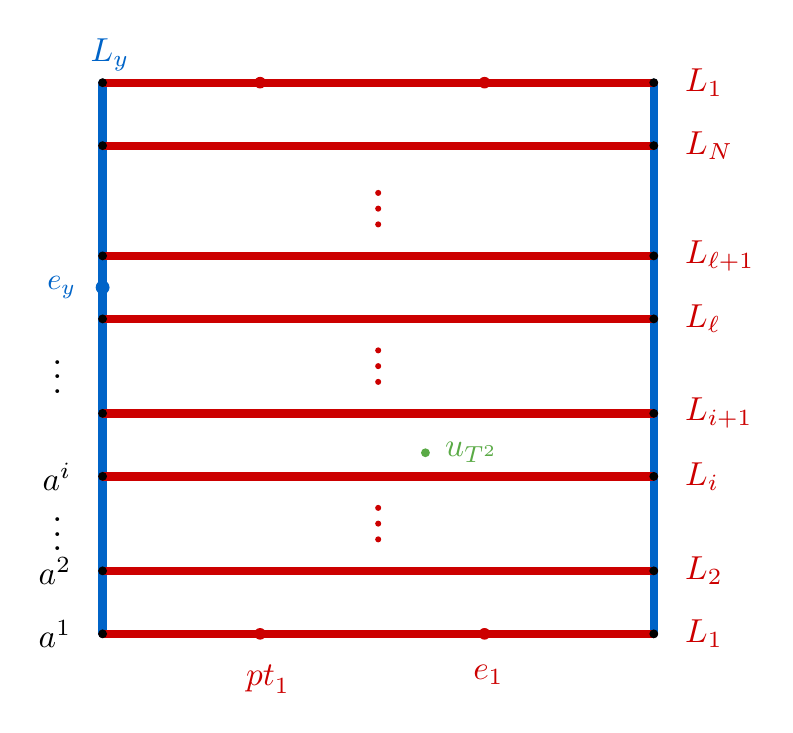
\begin{tikzpicture}[x=1cm,y=1cm, line cap=round, line join=round]
		
		% --- Colors
		\definecolor{myPurple}{RGB}{204,0,0}
		\definecolor{myOrange}{RGB}{0,100,200}
		\definecolor{myGreen}{RGB}{90,170,70}
		
		% --- Geometry (SQUARE)
		\def\xL{0}
		\def\xR{7}    % square: width = height = 7
		
		\def\yTop{7.0}
		\def\yAA{6.2}
		\def\yA{4.8}
		\def\yB{4}
		\def\yC{2.8}
		\def\yD{2}
		\def\yE{0.8}
		\def\yBot{0.0}
		
		% --- Orange vertical sides
		\draw[myOrange, line width=3pt] (\xL,\yBot) -- (\xL,\yTop);
		\draw[myOrange, line width=3pt] (\xR,\yBot) -- (\xR,\yTop);
		
		% --- Helper: horizontal line + endpoints
		\newcommand{\hlinewithdots}[1]{%
			\draw[myPurple, line width=3pt] (\xL,#1) -- (\xR,#1);
			\fill[black] (\xL,#1) circle (1.6pt);
			\fill[black] (\xR,#1) circle (1.6pt);
		}
		
		% --- Horizontal lines
		\hlinewithdots{\yTop}
		\hlinewithdots{\yAA}
		\hlinewithdots{\yA}
		\hlinewithdots{\yB}
		\hlinewithdots{\yC}
		\hlinewithdots{\yD}
		\hlinewithdots{\yE}
		\hlinewithdots{\yBot}
		
		% --- Interior points
		\fill[myPurple] (2.0,\yTop) circle (1.4pt);
		\fill[myPurple] (4.8,\yTop) circle (1.4pt);
		
		\fill[myPurple] (2.1,\yBot) circle (1.4pt);
		\fill[myPurple] (4.9,\yBot) circle (1.4pt);
		
		% --- Vertical dots
		\foreach \yy in {5.6,5.4,5.2} { \fill[myPurple] (3.5,\yy) circle (1.1pt); }
		\foreach \yy in {3.6,3.4,3.2} { \fill[myPurple] (3.5,\yy) circle (1.1pt); }
		\foreach \yy in {1.6,1.4,1.2} { \fill[myPurple] (3.5,\yy) circle (1.1pt); }
		
		% --- Left labels
		\node[myOrange, anchor=south west, scale=1.2] at (-0.3,\yTop) {$L_y$};
		
		\fill[myOrange] (\xL, {(\yA+\yB)/2}) circle (2.5pt);
		\node[myOrange, anchor=east, scale=1.1] at (-0.2, {(\yA+\yB)/2}) {$e_y$};
		
		\node[black, anchor=east, scale=1.2] at (-0.25,\yBot) {$a^1$};
		\node[black, anchor=east, scale=1.2] at (-0.25,\yE) {$a^2$};
		\node[black, anchor=east, scale=1.2] at (-0.25,\yD) {$a^i$};
		\node[black, anchor=east, scale=1.3] at (-0.35,{(\yE+\yD)/2}) {$\vdots$};
		\node[black, anchor=east, scale=1.3] at (-0.35,{(\yB+\yC)/2}) {$\vdots$};
		
		% --- Right labels
		\node[myPurple, anchor=west, scale=1.2] at (\xR+0.25,\yTop) {$L_1$};
		\node[myPurple, anchor=west, scale=1.2] at (\xR+0.25,\yAA) {$L_{N}$};
		\node[myPurple, anchor=west, scale=1.2] at (\xR+0.25,\yA) {$L_{\ell+1}$};
		\node[myPurple, anchor=west, scale=1.2] at (\xR+0.25,\yB) {$L_{\ell}$};
		\node[myPurple, anchor=west, scale=1.2] at (\xR+0.25,\yC) {$L_{i+1}$};
		\node[myPurple, anchor=west, scale=1.2] at (\xR+0.25,\yD) {$L_i$};
		\node[myPurple, anchor=west, scale=1.2] at (\xR+0.25,\yE) {$L_2$};
		\node[myPurple, anchor=west, scale=1.2] at (\xR+0.25,\yBot) {$L_1$};
		
		% --- Green point
		\fill[myGreen] (4.1,2.3) circle (1.6pt);
		\node[myGreen, anchor=west, scale=1.2] at (4.2,2.3) {$u_{\mathbb{T}^2}$};
		
		% --- Bottom labels
		\node[myPurple, anchor=north, scale=1.2] at (2.1,-0.25) {$\text{pt}_1$};
		\node[myPurple, anchor=north, scale=1.2] at (4.9,-0.25) {$e_1$};
		
		
		% --- Purple dots on top & bottom lines (interior)
		\fill[myPurple] (2,\yTop) circle (2.1pt);
		\fill[myPurple] (4.85,\yTop) circle (2.1pt);
		
		\fill[myPurple] (2,\yBot) circle (2.1pt);
		\fill[myPurple] (4.85,\yBot) circle (2.1pt);
		
	\end{tikzpicture}
	\caption{The fundamental domain of $\mathbb{T}^2$ with the approximating family of Lagrangians $\mathcal{N}(N)$ discussed in Proposition \ref{prop235}.} \label{fig:T2approx}
\end{figure}
%3D PICTURE
%\begin{figure}
%	\centering
%	\tdplotsetmaincoords{70}{115}
%	
%	\begin{tikzpicture}[tdplot_main_coords, line cap=round, line join=round, scale=1.25]
%		
%		% --- Colors (same as your figure)
%		\definecolor{myPurple}{RGB}{102,0,153}
%		\definecolor{myOrange}{RGB}{230,140,20}
%		
%		% --- Radii
%		\def\R{2.3}   % major radius
%		\def\r{0.85}  % minor radius
%		
%		% --- Styles
%		\tikzset{
%			purpleloop/.style={myPurple, line width=1.4pt},
%			orangeloop/.style={myOrange, line width=2.2pt},
%			faint/.style={black, opacity=0.18, line width=0.4pt},
%		}
%		
%		% (Optional) faint torus grid for 3D readability
%		\foreach \vv in {0,45,90,135} {
%			\draw[faint]
%			plot[variable=\uu, domain=0:360, samples=140]
%			({(\R+\r*cos(\vv))*cos(\uu)},
%			{(\R+\r*cos(\vv))*sin(\uu)},
%			{\r*sin(\vv)});
%		}
%		\foreach \uu in {0,60,120,180,240,300} {
%			\draw[faint]
%			plot[variable=\vv, domain=0:360, samples=140]
%			({(\R+\r*cos(\vv))*cos(\uu)},
%			{(\R+\r*cos(\vv))*sin(\uu)},
%			{\r*sin(\vv)});
%		}
%		
%		% --- Many PURPLE circles: fix v, vary u  (like horizontal lines in the square)
%		% --- Many PURPLE circles: fix v, vary u  (FULL 0..360 coverage)
%		\foreach \vv in {0,20,40,60,80,100,120,140,160,180,200,220,240,260,280,300,320,340} {
%			\draw[purpleloop]
%			plot[variable=\uu, domain=0:360, samples=180]
%			({(\R+\r*cos(\vv))*cos(\uu)},
%			{(\R+\r*cos(\vv))*sin(\uu)},
%			{\r*sin(\vv)});
%		}
%		
%		
%		% --- One ORANGE circle: fix u, vary v  (one vertical direction cycle)
%		\def\uOrange{35} % pick where it sits (degrees)
%		\draw[orangeloop]
%		plot[variable=\vv, domain=0:360, samples=220]
%		({(\R+\r*cos(\vv))*cos(\uOrange)},
%		{(\R+\r*cos(\vv))*sin(\uOrange)},
%		{\r*sin(\vv)});
%		
%	\end{tikzpicture}
%	\caption{AA}
%\end{figure}

\begin{proof}
	We assume that the critical point $u_{\mathbb{T}^2}$ doesn't lie on any Lagrangian in $\mathcal{N}(N)$. We denote by $e_j\in CF(L_j,L_j)$ and $\text{pt}_j\in CF(L_j,L_j)$ the maximum and the minimum of the Morse function $f_p^{L_j}$ for any $j=1,\ldots, N$. Moreover, for any $j$, we denote by $a^j_{xy}\in CF(L_j,L_y)$ and $a^j_{yx}\in CF(L_y,L_j)$ the intersection point $a$ seen as a generator of the Floer complexes. We denote by $i\in \{1,\ldots, N\}$ the unique index such that $u_{\mathbb{T}^2}$ lies in the area between $L_i$ and $L_{i+1}$. Similarly, we denote by $l$ the unique index such that $e_y\in CF(L_y,L_y)$ lies in the $L_y$-segment between $L_l$ and $L_{l+1}$. Figure \ref{fig:T2approx} provides a schematic depiction of the geometric setup.
	
	For any $j=1,\ldots, N$, consider the Hochschild chain\footnote{Here $N+1=1$.} $$\gamma^j:=a^j_{xy}\otimes a^{j+1}_{yx}\otimes a^{j+1}_{xy}\otimes a^{j}_{yx}\in CC_*(\mathcal{N}(N)).$$ Given a real number $A\in \mathbb{R}$, let\footnote{Here $h$ stands for \textit{horizontal} and $v$ for \textit{vertical.}} $$q^h_{A}(T):= \sum_{n,m>0}n(T^{n(m-1+A)}+ T^{n(m-A)}) \text{   and   } \tilde{q}^h_{\frac{1}{N}}(T):`= \sum_{n,m>0}T^{n(m-1+A)}+ T^{n(m-A)}$$ as well as 
	$$q^v_A(T):= \sum_{n,m>0}m(T^{n(m-A)}+ T^{n(m+A)}) \text{   and   } \tilde{q}^v_A(T):= \sum_{n,m>0}T^{n(m-A)}+ T^{n(m+A)} $$ be elements of the Novikov field $\Lambda$. We compute the Hochschild differential of $\gamma^j$ by computing all possible contractions. 
	\begin{enumerate}
		\item We have $$\mu_4(a^{j}_{xy},a^{j+1}_{yx}, a^{j+1}_{xy}, a^{j}_{yx}) = q^h_{\frac{1}{N}}(T)e_j\text{   and   } \mu_4(a^{j+1}_{xy},a^{j}_{yx},a^{j}_{xy},a^{j+1}_{yx})= q^h_{\frac{1}{N}}(T)e_{j+1},$$ while $$\mu_4(a^{j}_{yx},a^{j}_{xy},a^{j+1}_{yx}, a^{j+1}_{xy}) = \mu_4(a^{j+1}_{yx},a^{j+1}_{xy},a^{j}_{yx},a^{j}_{xy})= \begin{cases}
			q^v_{\frac{1}{N}}(T) e_y, \text{  if }j\neq l\\
			q^v_{1-\frac{1}{N}}(T)e_y, \text{  if }j=l.
		\end{cases} $$ %$$\mu_4(a^{j}_{yx},a^{j}_{xy},a^{j+1}_{yx}, a^{j+1}_{xy}) = \mu_4(a^{j+1}_{yx},a^{j+1}_{xy},a^{j}_{yx},a^{j}_{xy})= \begin{cases}                \sum_{n,m>0}m(T^{n(m-\frac{1}{N})}+ T^{n(m+\frac{1}{N})})e_y, \text{  if }j\neq l\\                \sum_{n,m>0}m(T^{n(m+\frac{1}{N}-1)}+ T^{n(m+1-\frac{1}{N})})e_y, \text{  if }j=l            \end{cases} $$ 
		\item We have $$\mu_3(a^{j}_{xy},a^{j+1}_{yx}, a^{j+1}_{xy}) = \tilde{q}^h_{\frac{1}{N}}(T)a^j_{xy} \text{   and   }\mu_3(a^{j+1}_{yx},a^{j+1}_{xy},a^{j}_{yx}) = \tilde{q}^h_{\frac{1}{N}}(T)a^{j}_{yx}$$
		while $$\mu_3(a^{j}_{yx},a^{j}_{xy},a^{j+1}_{yx}) = \tilde{q}^h_{\frac{1}{N}}(T)a^{j+1}_{yx} \text{   and   }\mu_3(a^{j+1}_{xy},a^j_{yx},a^{j}_{xy}) = \tilde{q}^h_{\frac{1}{N}}(T)a^{j+1}_{xy}$$
		
	\end{enumerate}
	We now compute the relevant $\mu_3$'s.
	It follows that \begin{align*}
		d_{CC}(\gamma^j) & = q^h_{\frac{1}{N}}(T)(e_j+e_{j+1}) + 2q^v_{c_j}(T)e_y + \tilde{q}^h_{\frac{1}{N}}(T)(2a^j_{xy}\otimes a^j_{yx} + a^{j+1}_{xy}\otimes a^{j+1}_{yx} + a^{j+1}_{yx}\otimes a^{j+1}_{xy}) \\ & = q^h_{\frac{1}{N}}(T)(e_j+e_{j+1}) + \tilde{q}^h_{\frac{1}{N}}(T)(a^{j+1}_{xy}\otimes a^{j+1}_{yx} + a^{j+1}_{yx}\otimes a^{j+1}_{xy})
	\end{align*}
	where $c_j = \frac{1}{N}$ if $j\neq l$ and $c_j=1-\frac{1}{N}$ otherwise.
	Hence $$d_{CC}\left(\sum_{j=1}^N \gamma^j\right) =  \tilde{q}^h_{\frac{1}{N}}(T)\sum_{j=1}^N(a^{j}_{xy}\otimes a^{j}_{yx} + a^{j}_{yx}\otimes a^{j}_{xy}) $$ as by summing over $j$ the summands of the form $e_j$ cancel out in pairs. In particular, $\sum_{j=1}^N\gamma^j$ is not a cycle. However, we claim that $$\vec{\gamma} = \sum_{j=1}^N\gamma^j + \tilde{q}^h_{\frac{1}{N}}(T)\ e_j\otimes a^j_{xy}\otimes a^j_{yx}\in CC_*(\mathcal{N}(N))$$ is a cycle. Indeed: $$d_{CC}(e_j\otimes a^j_{xy}\otimes a^j_{yx}) = \mu_2(e_j,a^j_{xy})\otimes a^j_{yx} + \mu_2(a^j_{yx},e_j)\otimes a^j_{xy} =a^{j}_{xy}\otimes a^{j}_{yx} + a^{j}_{yx}\otimes a^{j}_{xy},$$ since $e_j$ is a strict unit and the product of the point with itself vanishes.\\
	
	We now compute $OC^{\mathcal{N}(N)}(\vec{\gamma})\in CQ(\mathbb{T}^2)$. Recall that $i\in \{1,\ldots, N\}$ is defined as the only index such that the critical point $u=u_{\mathbb{T}^2}$ of the Morse function $f^{\mathbb{T}^2}_p$ used to define $QH_*(M)$ lies in the area between $L_i$ and $L_{i+1}$. Let $j\in \{1,\ldots, N\}$, then \begin{align*}
		OC(\gamma^j) &= \begin{cases}
			\sum_{n,m>0}nm(T^{n(m-\frac{1}{N})}+T^{n(m+\frac{1}{N})})u,  \text{ if }j\neq i\\
			\sum_{n,m>0}nm(T^{n(m-1+\frac{1}{N})}+T^{n(m+1-\frac{1}{N})})u,  \text{ if }j=i
		\end{cases}
	\end{align*}
	On the other hand, for all $j\in \{1,\ldots, N\}$ it is easy to see that we have $$OC(e_j\otimes a^j_{xy}\otimes a^j_{yx}) =0.$$ If $N$ is odd, then we have $$OC(\vec{\gamma}) = OC(\gamma^i) = \sum_{k\geq 0}\sum_{\substack{d=\pm 1 \ (2N)\\ d|2k+1}}T^{\frac{2k+1}{N}}$$ while if $N$ is even we have, for some $j\neq i$: $$OC(\vec{\gamma}) = OC(\gamma^i)+OC(\gamma^j) = \sum_{k\geq 0}\sum_{\substack{d=\pm 1, \pm1+N \ (2N)\\ d|2k+1}}T^{\frac{2k+1}{N}}$$
	%If $N$ is odd, then $$OC(\vec{\gamma}) = OC(\gamma^i)$$ since all other contributions cancel out over $\Z_2$. If $N$ is even, we have $$OC(\vec{\gamma}) = $$
	In all cases the lowest order term is $T^{\frac{1}{N}}u_{\mathbb{T}^2}$. The claim follows.
	
\end{proof}

%\begin{proof}[Proof of Theorem \ref{retractapproxt2}]	Let $\Delta>0$ and consider the family $\mathcal{N}=\{L_y\}\cup \{L_x^\theta \ : \ \theta \in S^1\}$ introduced above. We choose a subset $\mathcal{N}(N)$ of cardinality $N+1$ as in Proposition \ref{prop235}. Then for any filtered perturbation datum $p$ as in the proof of proposition \ref{prop235} of size $\nu(p)<\frac{1}{4}(\delta-\frac{1}{N})$, the family $\mathcal{L}^{we}(\mathbb{T}^2)$ of non-contractible Lagrangians on $\mathbb{T}^2$ is retract approximated by $\mathcal{N}(N)$ with accuracy $\delta$ in the TPC $\mathcal{C}\mathcal{F}uk(\mathbb{T}^2,p)$.\end{proof}

In Proposition \ref{prop235} we worked with only one Lagrangian in the $y$ direction. We can generalize the result to families containing $N+M$ circles, $N$ in the $x$ direction and $M$ in the $y$ direction, to get retract-approximation of order $\frac{1}{NM}$. Below we prove this for $N=M$.

\begin{prop}
	Let $p\in \mathcal{P}$ and $N\geq 1$. Consider the family $$\mathcal{N}(N)= \{L^1_y,\ldots, L_y^N,L_x^1,\ldots, L_x^N\}\subset \mathcal{N},$$ where $$L_y^j:= L_y^{\frac{j-1}{N}}\text{    and    }L_x^j=L_x^{\frac{j-1}{N}}$$ for $j=1,\ldots, N$. Then $\mathcal{N}(N)$ retract-approximates $\mathcal{L}^{we}(\mathbb{T}^2)$ with accuracy $\frac{1}{2N^2}+ 3\nu(p)$ in $\mathcal{A}_p$.
\end{prop}
\begin{proof}
	Essentially, the proof is the same as Proposition \ref{prop235}. We denote by $a^{j,k}$ the unique intersection point in $L_x^j\cap L_y^k$ and write it as $a^{j,k}_{xy}$ when seen as a generator of $CF(L_x^j,L_y^k)$ and as $a^{j,k}_{y,x}$ when seen as a generator of $CF(L_y^k,L_x^j)$. Let $i_x$ and $i_y$ the only indices such that the critical point $u=u_{\mathbb{T}^2}$ of the Morse function defining $QH(\mathbb{T}^2)$ lies in the square bounded by the Lagrangians $L_x^{i_x}$, $L_x^{i_x+1}$, $L_y^{i_y}$ and $L_y^{i_y+1}$. The key fact is that 
	\begin{align*}
		OC(a^{i_x,i_y}_{xy}\otimes a^{i_y,i_x+1}_{yx}\otimes a^{i_x+1,i_y+1}_{xy}\otimes a^{i_y+1,i_x}_{yx})&=\sum_{n,m>0}nm(T^{(n-1+\frac{1}{N})(m-1+\frac{1}{N}}+T^{(n+1-\frac{1}{N})(m+1-\frac{1}{N}})u \\& =\sum_{n>0}n^2(T^{(n-1+\frac{1}{N})^2}+T^{(n+1-\frac{1}{N})^2})u\\ & = \sum_{n\geq 0}T^{(2n+\frac{1}{N})^2}+T^{(2n+2-\frac{1}{N})^2}u\\ & = \sum_{n\in \mathbb{Z}}T^{(2n+\frac{1}{N})^2 }u= \theta_{\frac{1}{2N},0}(4,0)u
	\end{align*} In particular, the smallest exponent in this serie is $\frac{1}{N^2}$. One finishes the proof by showing that summing all possible cyclic combinations of tensors of intersection point plus some deformations involving the units in the Lagrangian Floer complex as in the proof of Proposition \ref{prop235} one gets a Hochschild cycle.
\end{proof}


%=======================================
%=======================================
%=======================================


\subsubsection{End of proof of Corollary \ref{S2T2}}

The proof of Corollary \ref{S2T2} is now a matter of packing the results of the last two sections.
\begin{proof}[Proof of Corollary \ref{S2T2}]
	We begin with the case of the sphere. 
	Let $\varepsilon_0>0$ and consider the family $\mathcal{E}\subset \lag^{\text{(mon,} \mathbf{0} \text{)}}(S^2)$ of straight equators passing through north and south pole introduced above. Let $N_0\geq 1$ such that $\frac{1}{4N_0}<\varepsilon_0$ and choose a subset $\mathcal{E}(N_0)\subset \mathcal{E}$ of cardinality $N_0$ as in Proposition \ref{OCS2}. Let $\delta_0:=\frac{1}{2}\left(\varepsilon_0-\frac{1}{4N_0}\right)$. Then for any perturbation datum $p$ as in the proof of Proposition \ref{OCS2} of size $\nu(p)<\delta_0$, the family $\lag^{\text{(mon,} \mathbf{0} \text{)}}(S^2)$ is $\varepsilon_0$-retract approximated by $\mathcal{E}(N_0)$ in $PD(\fuk(\lag^{\text{(mon,} \mathbf{0} \text{)}}(S^2);p))$. It follows that $\lag^{\text{(mon,} \mathbf{0} \text{)}}(S^2)$ is retract-approximable by $\mathcal{E}$ in the sense of Definition \ref{d:approx-sys-ret}. 
	\\ Let $\varepsilon_1>0$ and consider the family $\mathcal{N}\subset\lagwex(\mathbb{T}^2)$ introduced above. Let $N_1\geq 1$ such that $\frac{1}{2N_1}<\varepsilon_1$ and  choose a family $\mathcal{N}(N_1)$ of cardinality $N_1+1$ and containing $L_y$ as in Proposition \ref{prop235}. Let $\delta_1:= \frac{1}{3}(\varepsilon_1-\frac{1}{2N_1})$. Then for any perturbation datum as in te proof of Proposition \ref{prop235} of size $\nu(p)<\delta_1$, the family $\lagwex(\mathbb{T}^2)$ is $\varepsilon_1$-retract-approximable by $\mathcal{N}(N_1)$ in $PD(\fuk(\lagwex(\mathbb{T}^2);p))$. It follows that $\lagwex(\mathbb{T}^2)$ is retract-approximable by $\mathcal{N}$ in the sense of Definition \ref{d:approx-sys-ret}. \end{proof}

\subsection{Proof of Theorem \ref{thmmain1} ii and iii.}\label{subsec:proof_ThmAii}
Corollary \ref{S2T2} claims retract approximability in the sense of Definition \ref{d:approx-sys-ret} for the classes of Lagrangian submanifolds, $\lag^{\text{(mon,} \mathbf{0} \text{)}}(S^2)$ and $\lagwex(\mathbb{T}^2)$, that appear at the points ii and iii of Theorem \ref{thmmain1}. To conclude the proof of this theorem we need to remark that retract approximability in the sense of  Definition \ref{d:approx-sys-ret} implies retract approximability in the sense of Definition \ref{def:TPC-approx}. This argument has already been discussed in the proof of the point i of Theorem \ref{thmmain1}, in \S\ref{subsubsec:local_approx_d} but we will revisit it here.

First, notice that the approximating data $(\Phi, \F)$ is clear from the proof of Corollary \ref{S2T2}. For instance, for $\lag^{(mon,\bf{0})}(S^{2})$ the maps
$$\Phi_{\eta} : \lag^{(mon,\bf{0})}(S^{2})\longrightarrow \Ob (PD(\fuk(\lag^{\text{(mon,} \mathbf{0} \text{)}}(S^2);p)))$$ are Yoneda embeddings (with $\nu(p) < \eta$, small enough)
and $\F_{\epsilon}$ is a family of sufficiently many great circles going through the north
and south poles on $S^{2}$, as in Proposition \ref{OCS2}.

The only point that remains to be clarified is the relation between the spectral metric on the domain of $\Phi$ and the interleaving metric on the target of the maps $\Phi$.
This relationships is analogous to the one described in \S\ref{subsubsec:local_approx_d} but there 
are some adjustments. 
First, we need to provide a definition of the spectral metric $d_{\gamma}$ that applies to monotone Lagrangians as well as to weakly-exact Lagrangians, and not only to exact Lagrangians
as in \S\ref{subsubsec:local_approx_d}. This is well-known in the literature but, for completeness, we recall this definition here. Consider two Lagrangians that are Hamiltonian istotopic $L$, $L'$ (in one of the classes considered in Theorem \ref{thmmain1})  and a Hamiltonian $H:[0,1]\times M\to \R$ such that the Floer homology $HF(L,L';H)$ is defined. Because $L$ and $L'$ are Hamiltonian isotopic the PSS map  
$QH(L)\to HF(L,L';H)$ is well defined and we let $\gamma ([L];H)\in \R$ be the spectral
invariant in (the persistence module) $HF(L,L';H)$ of the PSS-image of the fundamental class $[L]\in QH(L)$.  We then put, see for instance \cite{Kis-Sh}:

$$d_{\gamma}(L,L')=\limsup_{||H||_{H}\to 0}\  \gamma([L]; H)+ \gamma([L];\overline{H})$$
where $\overline{H}$ is the inverse Hamiltonian $\overline{H}(t,x)=-H(1-t,x)$.
For exact Lagrangians this definition is equivalent to the one in \S\ref{subsubsec:local_approx_d}.
Moreover, the arguments in \S\ref{subsubsec:local_approx_d} -  and in particular, the identity (\ref{eq:equality_int})  and the arguments in \cite{BCZ:tpc} justifying it -  remain true in this context and they show that the maps $\Phi$  restricted to a Hamiltonian isotopy class  are quasi-isometric embeddings. Therefore, this completes the argument
in the case of $\lag^{\text{(mon,} \mathbf{0} \text{)}}(S^2)$ given that all the Lagrangians in this space are Hamiltonian isotopic to the standard equator.

Finally, we consider the space $\lagwex(\mathbb{T}^2)$. The spectral distance, given as above, 
is not defined for two $L$ and $L'$ that are not Hamiltonian isotopic. However, the interleaving type distance $\hat{D}_{int}(-,-)$ from \S\ref{subsubsec:local_approx_d} is defined  on all of
$\lagwex(\mathbb{T}^2)$ and, as explained before, it coincides with the spectral distance on each Hamiltonian isotopy class. Thus
by putting
$$d_{\gamma} (L,L'):= \hat{D}_{int} (L,L'), \forall \ \ L , L'\in \lagwex(\mathbb{T}^2)$$
the proof of Theorem \ref{thmmain1} is complete.

